\subsection{Jugend Innovativ}

"Jugend Innovativ ist Österreichs smartester Schulwettbewerb für innovative Ideen und fördert die besten Talente seit 1987." \cite{jugendinnovativ_tagline}.

Jugend Innovativ ist ein Wettbewerb, bei dem SchülerInnen ihre Ideen einreichen können. Die besten Ideen werden dann in die nächste Runde ausgewählt und können dort weitere Preise gewinnen. Die Ideen werden in den Kategorien ICT und Digital, Engineering, Science, Design, Entrepreneurship und Sustainability. \cite{jugendinnovativ_kategorien}.

Das Projektteam hat sich für die Kategorie Engineering entschieden, da diese am besten zum Projekt passt. Das Projektteam hat sich bis zum jetztigen Zeitpunkt für das Halbfinale qualifiziert und wartet momentan darauf, ob das Projekt in die nächste Runde kommt. Um sich für das Finale zu qualifizieren, musste das Projektteam einen etwa 20 Seitigen Projektbericht einreichen. Dieser Projektbericht wurde von den Projektmitgliedern selbst erstellt und beinhaltet alle Informationen über das Projekt. Um den Projektbericht anschaulicher zu gestalten, wurde mittels CINEMA 4D ein Render des Turms erstellt. Dieser Render wurde als Deckblatt verwendet und ist in Abbildung \ref{fig:turm_visualisierung}.

\begin{figure}[H]
  \centering
  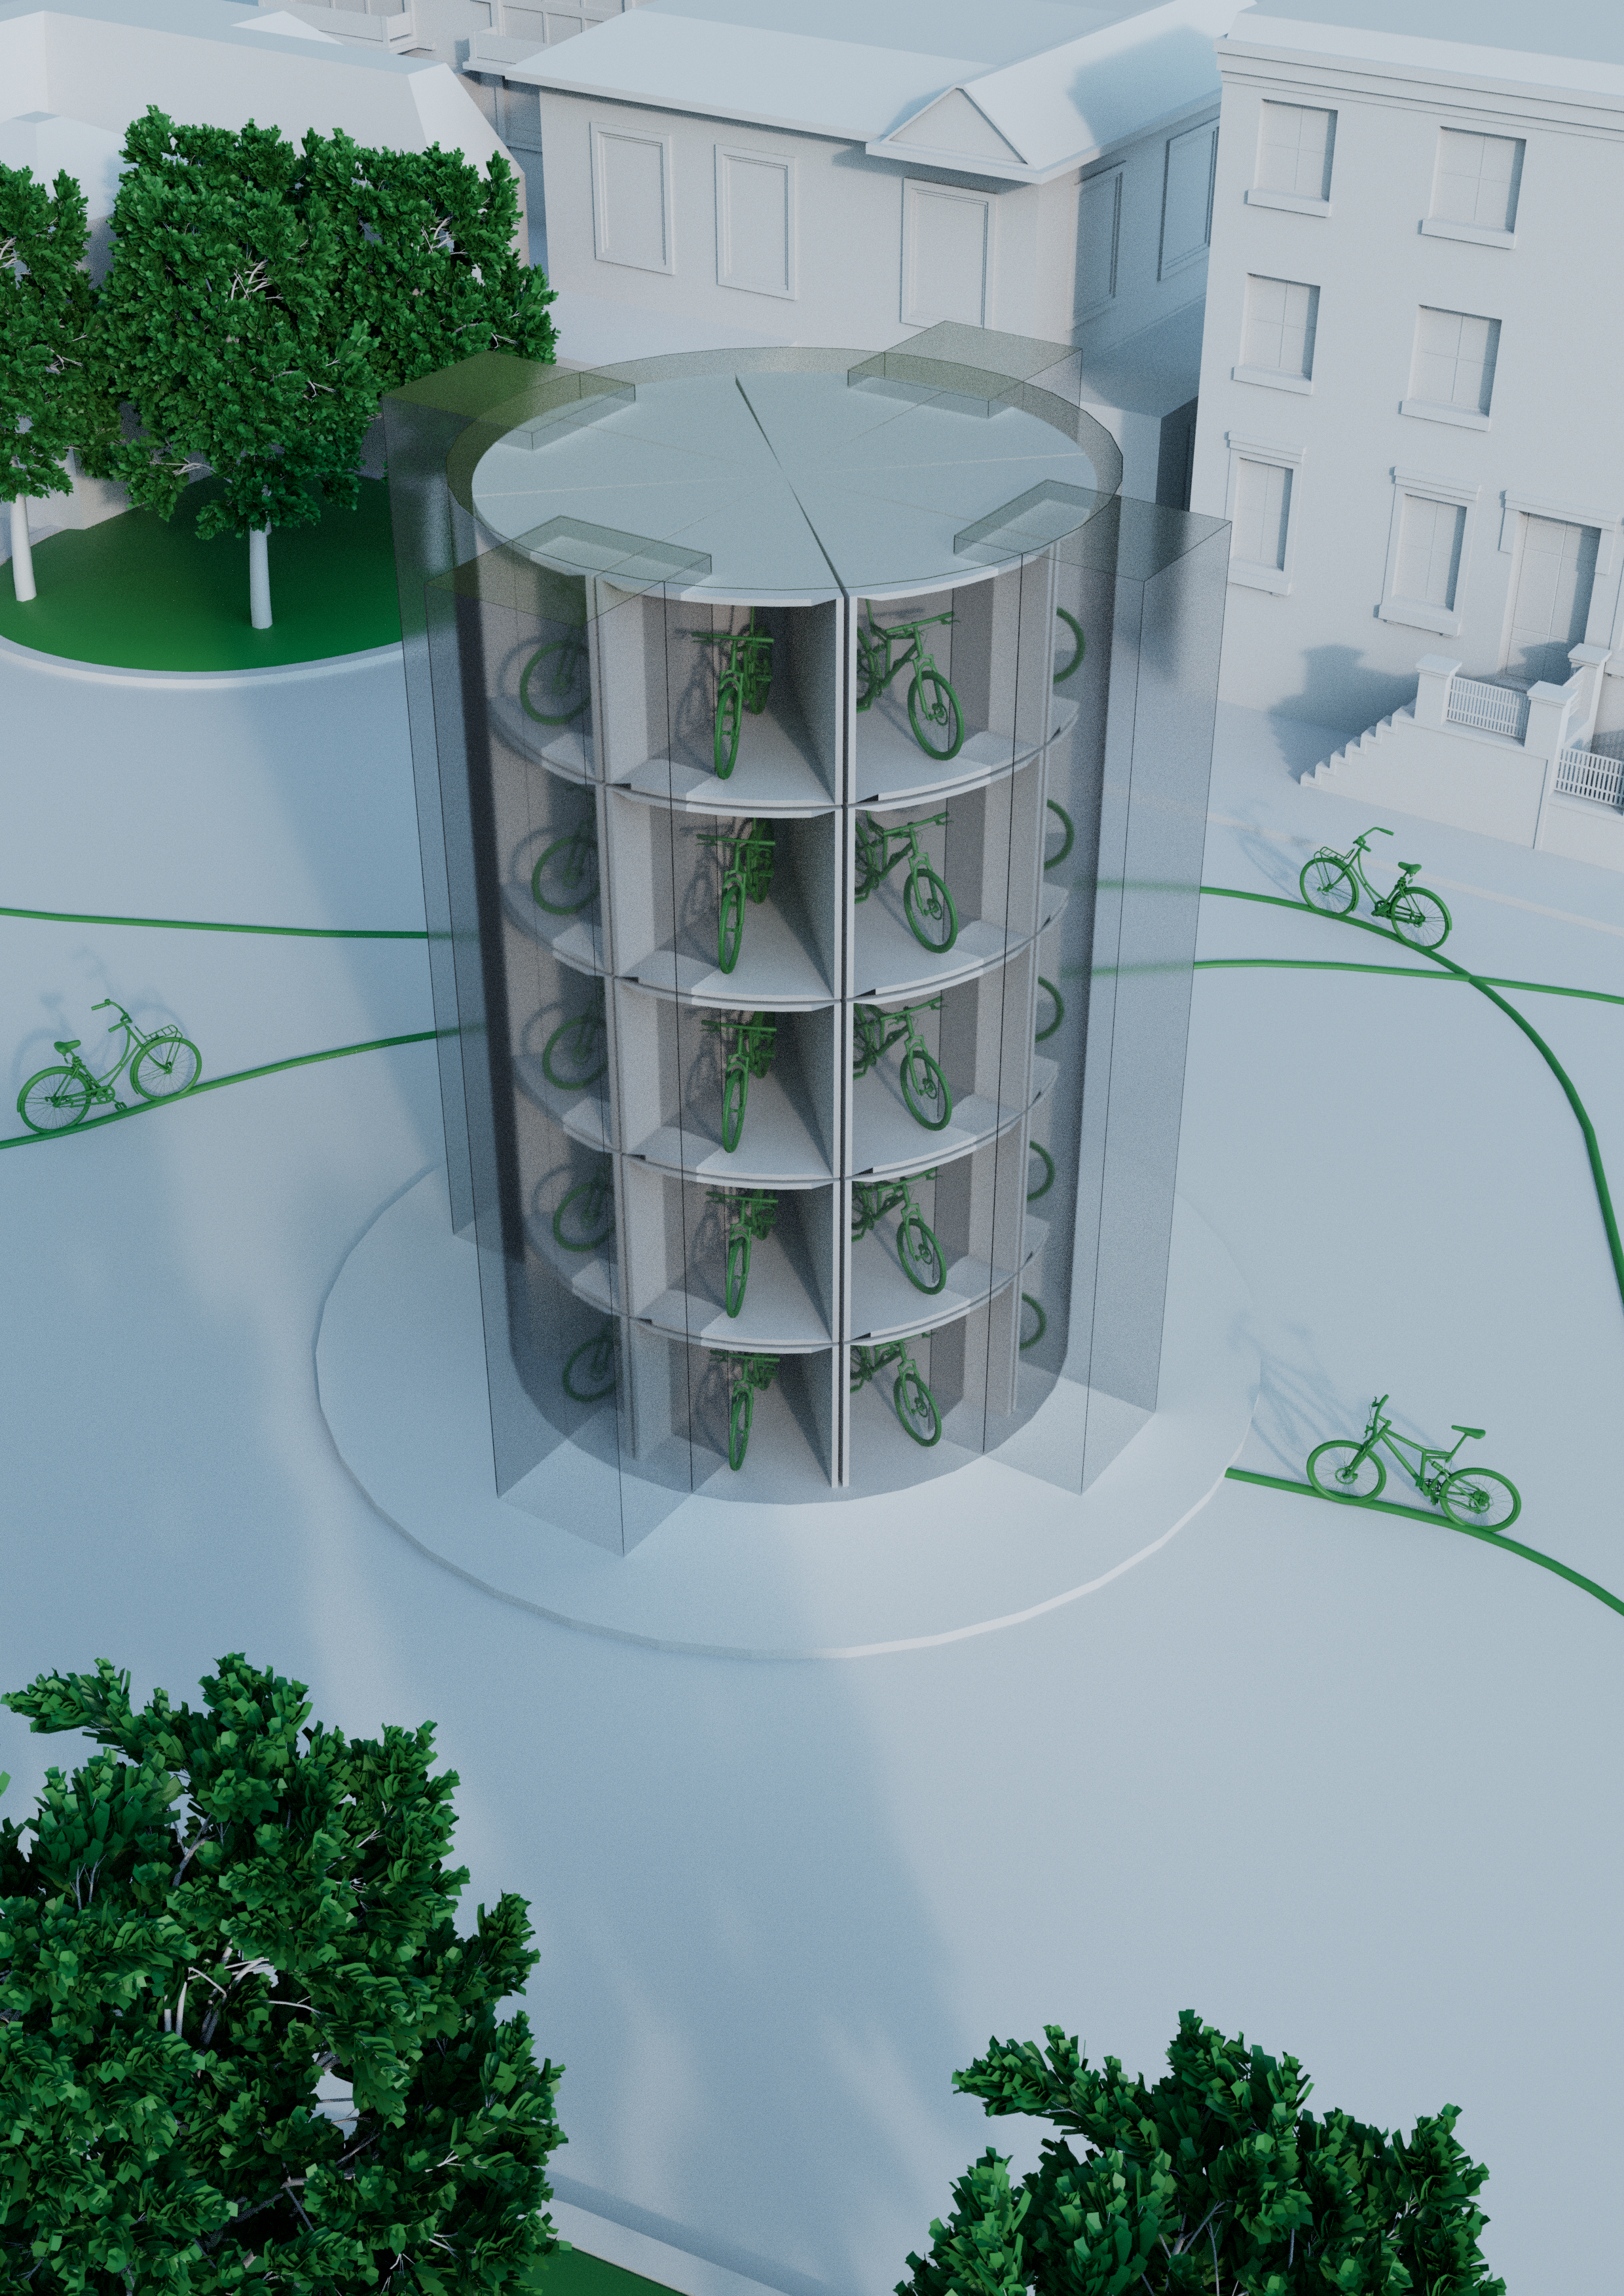
\includegraphics[width=0.6\textwidth]{images/turm_visualisierung.png}
  \caption{Visualisierung des Turms im Projektbericht}
  \label{fig:turm_visualisierung}
\end{figure}